\documentclass[a4paper,11pt]{article}
\usepackage[utf8]{inputenc}
\usepackage{amsmath}
\usepackage{amsfonts}
\usepackage{amssymb}
\usepackage{graphicx}
\usepackage{braket}

\numberwithin{equation}{section}
\renewcommand\thesubsection{\alph{subsection}}
\newcommand{\bvp}[1]{\mathbf{#1}'}
\newcommand{\bv}[1]{\mathbf{#1}}
\newcommand{\ez}{\epsilon_0}
\newcommand{\lrp}[1]{\left({#1}\right)}
\newcommand{\lrb}[1]{\left\{{#1}\right\}}


%opening
\title{Electromagnetic Theory I HW2}
\author{Vince Baker}

\begin{document}

\maketitle

\section{Problem 1.5}
We calculate the charge density directly from the Poisson equation, noting that the charge distribution is a function of $r$ only due to the spherical symmetry of the potential.
\begin{align}
 \nabla^2\Phi &= -\frac{\rho}{\ez}\\
 \Phi(r) &= \frac{q}{4\pi\ez}\frac{e^{-\alpha r}}{r}\left(1+\frac{\alpha r}{2} \right)\\
 \frac{\partial \Phi(r)}{\partial r} &= \frac{q}{4\pi\ez}\lrb{-\frac{\alpha e^{-\alpha r}}{r}-\frac{e^{-\alpha r}}{r^2}-\frac{\alpha^2}{2}e^{-\alpha r}}\\
 \nabla^2\Phi(r) &= -\frac{q}{4\pi\ez}\frac{1}{r^2}\frac{\partial}{\partial r}\lrb{r\alpha e^{-\alpha r}+e^{-\alpha r}+\frac{\alpha^2}{2}r^2e^{-\alpha r}}\\ 
 \nabla^2\Phi(r) &= \frac{q}{4\pi\ez}\frac{\alpha^3}{2}e^{-\alpha r}\\
 \rho(r) &= -\frac{q}{8\pi}\alpha^3e^{-\alpha r}
\end{align}
However, since the potential includes a $1/r$ factor it is not well-behaved at $r=0$. 
Solving for the Laplacian of the potential when $r=0$:
\begin{align}
 \nabla^2\Phi(r=0) &= \frac{q}{4\pi\ez}\nabla^2(\frac{1}{r})\\
 \nabla^2\Phi(r=0) &= -\frac{q}{\ez}\delta(r)\\
 \rho(r) &= q\delta(r)
\end{align}
So we see that the charge distribution is a combination of a positive point charge at the origin (proton) and the electron's negative effective charge distribution.

\section{Problem 1.6}
a) For the parallel plates we can see that the field inside must be uniform by the symmetry (we ignore the fringing fields since the plates are described as large).
Using a small Gaussian pillbox, we calculate that the field on the positive plate with charge density $\sigma = Q/A$ due to a differential area $dA$ is:
\begin{align}
 \int_S \bv{E} \cdot dA &= \frac{Q}{A\ez}\\
 \bv{E} &= \frac{Q}{A\ez}
\end{align}
Since the total flux through the top and bottom of the pillbox is $\frac{Q}{A\ez}$, the field pointing between the plates must be $\frac{Q}{2A\ez}$.
The field on the corresponding section of the negative plate is the same magnitude since both plates have the same area and total charge magnitude.
The sign is the same, since the normal to the negative plate surface points in the opposite direction but the sign of the charge is also reversed.
Therefore, the total field on a line between the two plates is:
\begin{align}
 \bv{E} &= \frac{Q}{A\ez}\hat{n}
\end{align}
Integrating this constant field along a line of length $d$ gives a potential difference $\frac{Qd}{A\ez}$.
The capacitance is the ratio of charge to potential, or:
\begin{align}
 C &= \frac{A\ez}{d}
\end{align}
\\
b) The field between the two spheres is entirely due to the charge Q on the inner sphere, and is:
\begin{align}
 \bv{E} &= \frac{1}{4\pi\ez}\frac{Q}{r^2}\hat{n}
\end{align}
Integrating this along any radial vector from a to b we find the potential difference:
\begin{align}
 V &= \int_a^b \frac{1}{4\pi\ez}\frac{Q}{r^2} dr\\
 V &= \frac{Q}{4\pi\ez}\lrb{-\frac{1}{b}+\frac{1}{a}}
\end{align}
The capcitance is then:
\begin{align}
 C &= \frac{Q}{V} = \frac{4\pi\ez}{1/a-1/b}
\end{align}
\\
c) The field between the cylinders will again come entirely from the charge Q on the inner cylinder of surface area $2\pi a L$ (we neglect the ends for a cylinder much longer than its radius).
Using Gauss' law:
\begin{align}
 \int_S \bv{E}\cdot d\bv{a} &= \frac{Q}{\ez}\\
 2\pi r L \bv{E} &= \frac{Q}{\ez}\\
 \bv{E} &= \frac{Q}{2\pi r L\ez} \hat{n}
\end{align}
Integrating on any radial to find the potential:
\begin{align}
 V &= \int_a^b \frac{Q}{2\pi r L\ez} dr\\
 V &= \frac{Q}{2\pi L\ez} \lrb{\ln{b}-\ln{a}}
\end{align}
The capacitance is then:
\begin{align}
 C &= \frac{Q}{V} = \frac{2\pi L\ez}{\ln{(b/a)}}
\end{align}
\\
d) Rearranging (6) to find $b$:
\begin{align}
 b = a e^{2\pi L\ez /C}
\end{align}
With the capacitance given in Farad/meter, we take the length as 1 meter. 
We then calculate b=6.4 mm for a capacitance of $3e^{-11}$ and b=113 km for a capacitance of $3e^{-12}$. 

\section{Problem 1.8}
a) We use equation 1.62 in Jackson for two conductors. 
We define the potential to be 0 on the lower-potential conductor, so that the total energy is $W=\frac{1}{2}Q\Delta V$.
We have already determined the potential difference when charges -Q, +Q are placed on the conductors:
\begin{align} 
 V_{plates} &= \frac{Qd}{A\ez}\\
 V_{spheres} &= \frac{Q}{4\pi\ez}\lrb{\frac{1}{a}-\frac{1}{b}}\\
 V_{cylinder} &= \frac{Q}{2\pi L\ez}\ln{\lrp{b/a}}
\end{align}
We can now solve for the total electrostatic energy:
\begin{align}
 W_{plates} &= \frac{Q^2d}{2A\ez}\\
 W_{spheres} &= \frac{Q^2}{8\pi\ez}\lrb{\frac{1}{a}-\frac{1}{b}}\\
 W_{cylinder} &= \frac{Q^2}{4\pi L\ez}\ln{\lrp{b/a}}
\end{align}
The energy in terms of potential difference can be foudn by rearranging equations 1-3 for Q, then inserting into Jackson 1.62.
\begin{align}
 W_{plates} &= \frac{A\ez V^2}{2d}\\
 W_{spheres} &= \frac{2\pi\ez V^2}{\lrb{\frac{1}{a}-\frac{1}{b}}}\\
 W_{cylinder} &= \frac{\pi L \ez V^2}{\ln{\lrp{b/a}}}
\end{align}
b) The electric field energy density along the lines of integration used to determine the potential difference are:
\begin{align}
 w_{plates} &= \frac{Q^2}{2\ez A^2}\\
 w_{spheres} &= \frac{Q^2}{32\pi^2\ez r^4}\\
 w_{cylinders} &= \frac{Q^2}{8\pi^2L^2\ez r^2}
\end{align}

The electric field energy density along the lines of integration used to determine the potential difference are sketched below.
We choose linear dimensions such that $a=1$ and $b=2$.
For the plates, our energy units are such that $\frac{Q^2}{2\ez A^2}=1$.
For the spheres, our energy units are such that $\frac{Q^2}{32\pi^2\ez}=1$.
For the cylinders, our energy units are such that $\frac{Q^2}{8\pi^2L^2\ez}=1$.
\begin{figure}[h]
 \caption{Electrostatic energy densities}
 \centering
   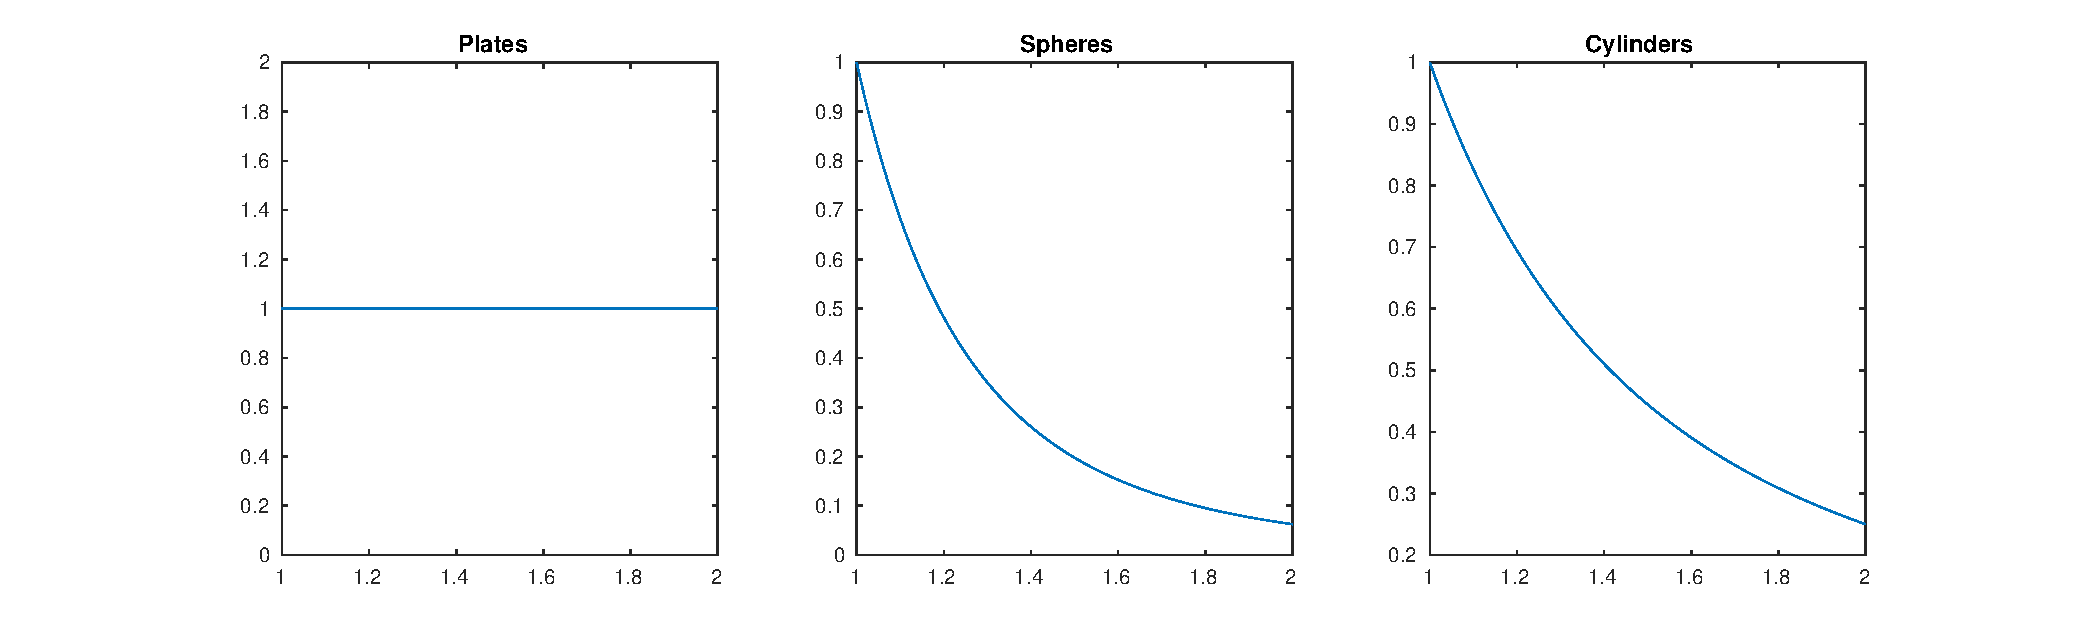
\includegraphics[width=\textwidth]{EnergyDensities}
\end{figure}



\end{document}
